From the given inequalities,
\begin{align}
    \myvec{-1&-2 \\ -2&-1 \\ 1&0 \\ 0&1}\vec{x} \succeq \myvec{-8 \\ -8 \\ 0 \\ 0}
\end{align}
Which can be further written as
\begin{align}
   \myvec{-1&-2 \\ -2&-1 }\vec{x} \succeq \myvec{-8 \\ -8} 
\end{align}
Let $u_1 \ge 0, u_2 \ge 0$.  This may be expressed as
\begin{align}
\vec{u} = \myvec{u_1\\u_2}\succeq \vec{0}
\end{align}
Now we have,
\begin{align}
  \myvec{-1&-2 \\ -2&-1 }\vec{x} \succeq \myvec{-8 \\ -8}  + \vec{u} 
\end{align}
\begin{align}
        \vec{x} = \myvec{-1 & -2 \\ -2 & -1}^{-1}\myvec{-8 \\ -8} + \myvec{-1 & -2 \\ -2 & -1}^{-1}\vec{u}
        \\
        \implies \vec{x} = \frac{-1}{3}\myvec{8 \\ 8}+\frac{-1}{3}\myvec{-1&2 \\ 2&-1}\vec{u}
        \\
        \vec{x}=\myvec{\frac{-8}{3} \\ \frac{-8}{3}}+\frac{-1}{3}\myvec{-1&2 \\ 2&-1}\vec{u}
    \end{align}
Thus the solution of the system of inequalities can be determined graphically, which is represented in Fig.     \ref{sep/2/4/Graphical solution}
\begin{figure}[ht]
    \centering
    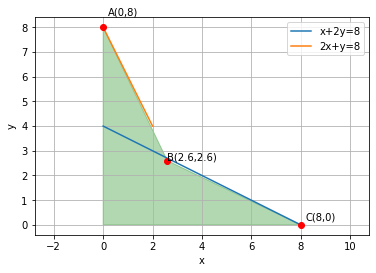
\includegraphics[width=\columnwidth]{solutions/sep/2/4/download.png}
    \caption{Graphical solution}
    \label{sep/2/4/Graphical solution}
\end{figure}


